\section{Motivation}\label{motivation}

\begin{frame}{What is Shor's algorithm?}

\begin{block}{A quantum algorithm for integer factorization}

\begin{itemize}
\item
  Quantum algorithm

  \begin{itemize}
  \itemsep1pt\parskip0pt\parsep0pt
  \item
    An algorithm that runs on quantum computers
  \end{itemize}
\item
  Integer factorization

  \begin{itemize}
  \item
    Decomposition of a composite number into smaller non-trivial
    divisors
  \item
    Example

    \begin{itemize}
    \itemsep1pt\parskip0pt\parsep0pt
    \item
      Given 24 , find its prime factor
    \item
      24 = $2^{3}\times 3$.
    \item
      Prime factor is 2, 3
    \end{itemize}
  \end{itemize}
\end{itemize}

\end{block}

\end{frame}

\begin{frame}{Why Shor's algorithm?}

\begin{block}{Faster}

\begin{itemize}
\item
  RSA

  \begin{itemize}
  \item
    Cryptosystem
  \item
    Widely used for secure data transmission
  \item
    Principle

    \begin{itemize}
    \item
      Easy to multiply prime numbers $\rightarrow$ Encryption
    \item
      Impossible to factor prime numbers $\rightarrow$ Decryption
    \end{itemize}
  \end{itemize}
\item
  Why not classical algorithm?

  \begin{itemize}
  \item
    Trial division

    \begin{itemize}
    \itemsep1pt\parskip0pt\parsep0pt
    \item
      Find if n can be divided by each number in turn that is less than
      n
    \end{itemize}
  \item
    Too slow

    \begin{itemize}
    \itemsep1pt\parskip0pt\parsep0pt
    \item
      Take $10^{176}$ years to factoring a 400-digit number.
    \end{itemize}
  \end{itemize}
\end{itemize}

\end{block}

\end{frame}

\begin{frame}{Why Shor's algorithm?}

\begin{block}{Embodiment of human ingenuity}

\begin{itemize}
\itemsep1pt\parskip0pt\parsep0pt
\item
  Math

  \begin{itemize}
  \itemsep1pt\parskip0pt\parsep0pt
  \item
    Euclidean algorithm 300 BC
  \item
    Chinese remainder theorem 300-500 AD
  \item
    Euler's theorem 1736
  \item
    Fast Fourier transform(Cooley-Tukey) 1965
  \end{itemize}
\item
  Physics

  \begin{itemize}
  \itemsep1pt\parskip0pt\parsep0pt
  \item
    Quantum physics 1900-Now
  \end{itemize}
\item
  Computer science

  \begin{itemize}
  \itemsep1pt\parskip0pt\parsep0pt
  \item
    Divide \& Conquer algorithm 1946
  \end{itemize}
\end{itemize}

\end{block}

\end{frame}

\section{Overview}\label{overview}

\begin{frame}{Overview}

\begin{block}{4 reductions of a complex problem}

\begin{itemize}
\itemsep1pt\parskip0pt\parsep0pt
\item
  Factoring is reduced to finding a nontrivial square root of 1 modulo N
\item
  Computing the order of a random integer modulo N
\item
  Find the period of a periodic superposition
\item
  Found by quantum FFT
\end{itemize}

\end{block}

\begin{block}{The tricks and secret of Shor's algorithm}

\begin{itemize}
\itemsep1pt\parskip0pt\parsep0pt
\item
  Tricks

  \begin{itemize}
  \itemsep1pt\parskip0pt\parsep0pt
  \item
    Number theory

    \begin{itemize}
    \itemsep1pt\parskip0pt\parsep0pt
    \item
      Classical computer
    \end{itemize}
  \end{itemize}
\item
  Secret

  \begin{itemize}
  \itemsep1pt\parskip0pt\parsep0pt
  \item
    Quantum FFT

    \begin{itemize}
    \itemsep1pt\parskip0pt\parsep0pt
    \item
      Quantum algorithm
    \end{itemize}
  \end{itemize}
\end{itemize}

\end{block}

\end{frame}

\begin{frame}{What is QFT?}

\begin{itemize}
\itemsep1pt\parskip0pt\parsep0pt
\item
  Fourier transform
\item
  $\downarrow$ In discrete domain
\item
  Discrete Fourier transform
\item
  $\downarrow$ Plus Divide \& Conquer algorithm
\item
  Fast Fourier transform
\item
  $\downarrow$ Modification for quantum computer
\item
  Quantum Fourier transform

  \begin{itemize}
  \itemsep1pt\parskip0pt\parsep0pt
  \item
    Quantum implementation of FFT
  \end{itemize}
\end{itemize}

\end{frame}

\section{Fourier transform}\label{fourier-transform}

\begin{frame}{What is Fourier transform?}

\begin{block}{Fourier series \& Fourier coeffcients}

\begin{itemize}
\item
  In 1807, Fourier astounded some of his contemporaries by asserting
  that an ``arbitrary'' function could be expressed as a linear
  combination of sines and cosines.
\item
  Amazingly, it's true.
\item
  Fourier series.

  \begin{itemize}
  \item
    $f(x) = \sum_{k=-\infty}^{\infty} c_{k}sinkx+\sum_{k=-\infty}^{\infty} c_{k}' coskx$
  \item
    Apply Euler's identity $e^{ix}=cosx+isinx$
  \item
    $f(x)=\sum_{-\infty}^{\infty} c_{k}e^{ikx}$
  \item
    $c_{k} = \frac{1}{2\pi}\int_{-\pi}^{\pi} f(x)e^{-ikx} dx$

    \begin{itemize}
    \itemsep1pt\parskip0pt\parsep0pt
    \item
      $c_{k}$ is called the $k^{th}$ Fourier coefficient of $f(x)$
    \end{itemize}
  \end{itemize}
\end{itemize}

\end{block}

\end{frame}

\begin{frame}{Does it work?}

\begin{block}{Two vital questions}

\begin{itemize}
\item
  Question: Given any reasonable function $f(x)$ on
  $\left[-\pi,\pi\right]$, with Fourier coefficients defined above, is
  it true that \[f(x) = \sum_{k=-\infty}^{\infty}c_{k}e^{ikx}?\]

  \begin{itemize}
  \itemsep1pt\parskip0pt\parsep0pt
  \item
    Yes
  \end{itemize}
\item
  Question: Are two functions with the same Fourier coefficients
  necessarily equal?

  \begin{itemize}
  \itemsep1pt\parskip0pt\parsep0pt
  \item
    Yes
  \end{itemize}
\end{itemize}

\end{block}

\end{frame}

\begin{frame}{The idea behind Fourier Transform}

\begin{block}{Analysis \& Synthesis}

\begin{itemize}
\itemsep1pt\parskip0pt\parsep0pt
\item
  Net force \& Components force
\end{itemize}

\centerline{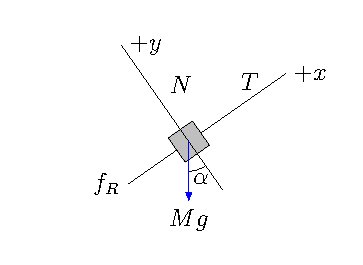
\includegraphics[width=1.3in]{b.eps}}

\begin{itemize}
\itemsep1pt\parskip0pt\parsep0pt
\item
  Fourier basis
\end{itemize}

\begin{tabular}{ccc}
  $\hat{\tmmathbf{v}}^1 = \frac{1}{\sqrt{N}} \left(\begin{array}{c}
    1\\
    1\\
    1\\
    \vdots\\
    1
  \end{array}\right)$, & $\hat{\tmmathbf{v}}^2 = \frac{1}{\sqrt{N}}
  \left(\begin{array}{c}
    1\\
    \zeta^2\\
    \zeta^3\\
    \vdots\\
    \zeta^{N - 1}
  \end{array}\right)$, & $\hat{\tmmathbf{v}}^3 = \frac{1}{\sqrt{N}}
  \left(\begin{array}{c}
    1\\
    \zeta^{2 \cdot 2}\\
    \zeta^{3 \cdot 2}\\
    \vdots\\
    \zeta^{( N - 1) \cdot 2}
  \end{array}\right)$,
\end{tabular}

\end{block}

\end{frame}

\section{Discrete Fourier transform}\label{discrete-fourier-transform}

\begin{frame}{Discrete Fourier transform}

\begin{block}{What if we do not know $F$?}

\begin{itemize}
\item
  Example: Given audio signals, continuous signals are sampled at
  discrete time intervals
\item
  Question: Given sample points, how to find Fourier coefficients?
\end{itemize}

\end{block}

\begin{block}{Consequence of sampling}

\begin{itemize}
\itemsep1pt\parskip0pt\parsep0pt
\item
  Aliasing
\end{itemize}

\centerline{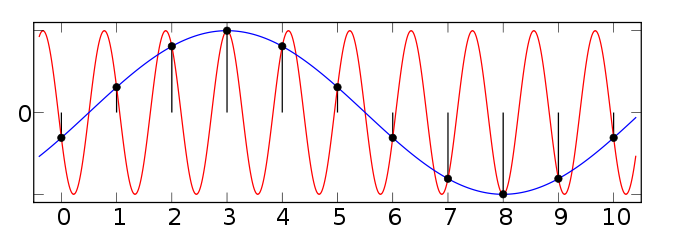
\includegraphics[width=3in]{aaa.png}}

\end{block}

\end{frame}

\begin{frame}{Discrete Fourier transform}

\begin{block}{Consequence of Aliasing}

\begin{itemize}
\itemsep1pt\parskip0pt\parsep0pt
\item
  We are allowed to represent $f(x)$ by a finite linear combination,
  which agrees on the sample points
\end{itemize}

\[f(x)\sim p(x)\]
\[f(x) = c_{0}+c_{1}e^{ix}+c_{2}e^{2ix}+\ldots+c_{n-1}e^{(n-1)ix}=\sum_{k=0}^{n-1}c_{k}e^{ikx}\]
\[\mathbf{f} = c_{0}\mathbf{\omega_{0}}+c_{1}\mathbf{\omega_{1}}+ \ldots + c_{n-1}\mathbf{\omega_{n-1}}\]
\[\mathbf{\omega_{k}}=(e^{ikx_{0}},e^{ikx_{1}},\ldots,e^{ikx_{n-1}})^{T}\]
\[\mathbf{\omega_{k}} = (1,\zeta_{n}^{k},\zeta_{n}^{2k},\ldots,\zeta_{n}^{(n-1)k})^{T}\]

\end{block}

\end{frame}

\begin{frame}{Notation}

\begin{itemize}
\itemsep1pt\parskip0pt\parsep0pt
\item
  Notation $\zeta_{m} = \sqrt[m]{1}$

  \begin{itemize}
  \itemsep1pt\parskip0pt\parsep0pt
  \item
    Fact $\zeta_{m}=\zeta_{n}^{2}$, when $n = 2m$
  \item
    Example $\zeta_{4}=\zeta_{8}^{2}$
  \end{itemize}
\end{itemize}

\centerline{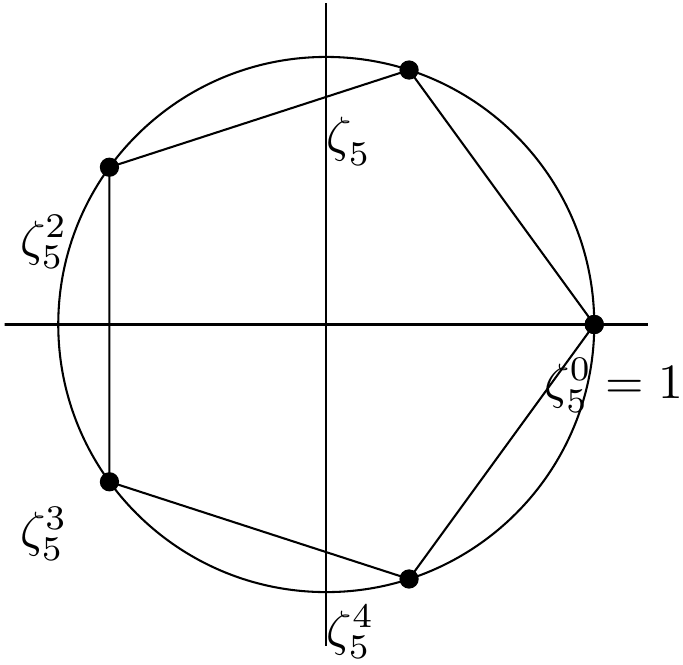
\includegraphics[width=2.25in]{bbb.png}}

\end{frame}

\section{Fast Fourier transform}\label{fast-fourier-transform}

\begin{frame}{Fast Fourier transform}

\begin{block}{Mathematical approach}

\begin{align*}
 c_{k}& =  \sum_{n=0}^{n-1} \zeta_{N}^{-nk}f_{n} \\
  & =  \sum_{n=0}^{N/2-1} \zeta_{N}^{2nk}f_{2n} + \sum_{n=0}^{N/2-1} \zeta_{N}^{k(2n+1)} f_{2n+1} \\
 & =  \sum_{n=0}^{N/2-1} \zeta_{N}^{2nk}f_{2n} + \zeta_{N}^{k}\sum_{n=0}^{N/2-1} \zeta_{N}^{2nk} f_{2n+1} \\
& = \sum_{n=0}^{N/2-1} \zeta_{N/2}^{nk}f_{2n} + \zeta_{N}^{k}\sum_{n=0}^{N/2-1} \zeta_{N/2}^{nk} f_{2n+1}
\end{align*}

\end{block}

\end{frame}

\begin{frame}{Fast Fourier transform}

\begin{block}{Visualization}

\centerline{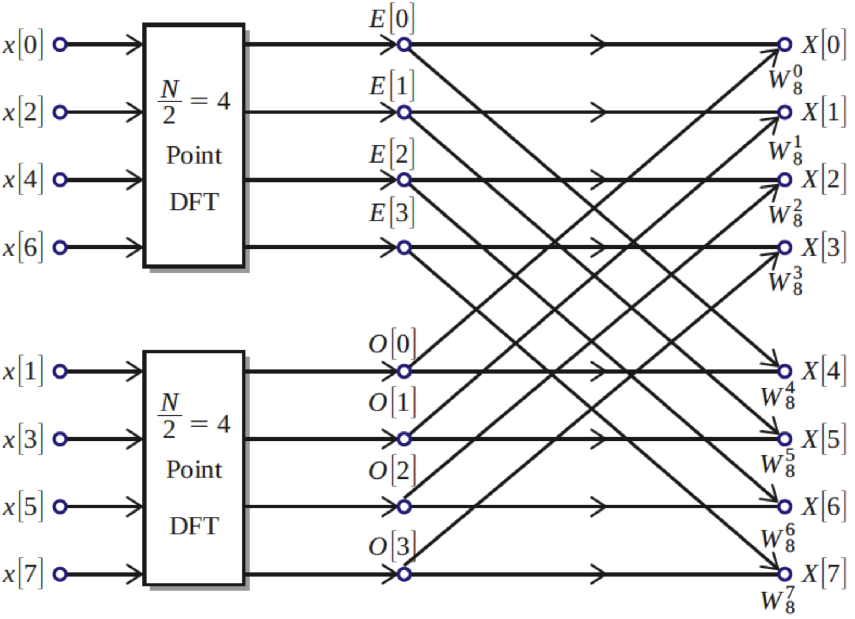
\includegraphics[width=3in]{c.png}}

\end{block}

\end{frame}

\begin{frame}{Fast Fourier transform}

\begin{block}{Divide \& Conquer}

\centerline{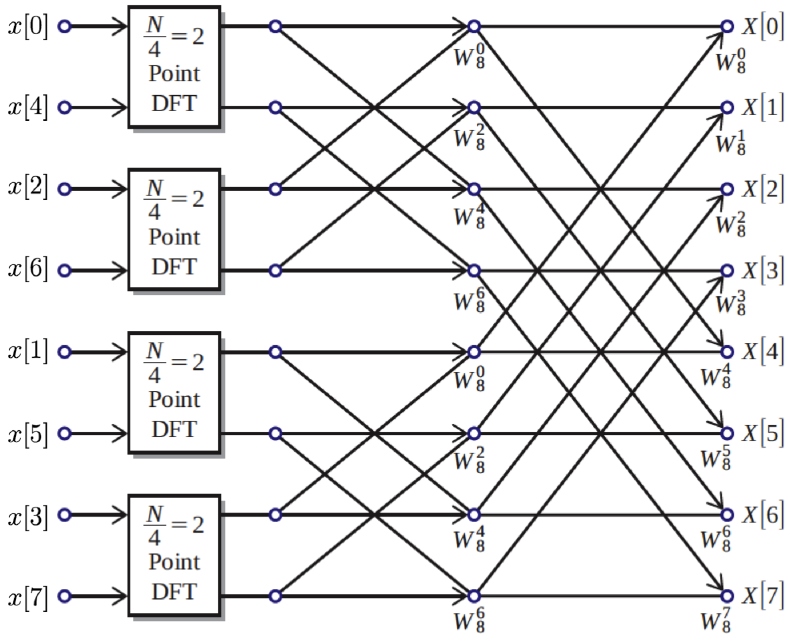
\includegraphics[width=3in]{cc.png}}

\end{block}

\end{frame}

\section{Quantum Fourier transofm}\label{quantum-fourier-transofm}

\begin{frame}{Qubits, superposition, measurement}

\begin{block}{Qubits \& Superposition}

\begin{itemize}
\itemsep1pt\parskip0pt\parsep0pt
\item
  Ordinary bits

  \begin{itemize}
  \itemsep1pt\parskip0pt\parsep0pt
  \item
    Electron
  \item
    Ground state \& excited state, 0 \& 1
  \end{itemize}
\item
  Quantum bits

  \begin{itemize}
  \itemsep1pt\parskip0pt\parsep0pt
  \item
    $|0 \rangle$, $|1 \rangle$
  \end{itemize}
\item
  Superposition

  \begin{itemize}
  \itemsep1pt\parskip0pt\parsep0pt
  \item
    $\alpha |0 \rangle + \beta |1 \rangle$
  \end{itemize}
\item
  Measurement

  \begin{itemize}
  \itemsep1pt\parskip0pt\parsep0pt
  \item
    Goal: determine which state
  \item
    Outcome: 0 or 1
  \item
    Disturbs the system
  \end{itemize}
\end{itemize}

\end{block}

\end{frame}

\begin{frame}{QFT?}

\begin{block}{QFT is quantum version of FFT}

\end{block}

\begin{block}{Why QFT?}

\begin{itemize}
\itemsep1pt\parskip0pt\parsep0pt
\item
  Extremely fast
\end{itemize}

\end{block}

\begin{block}{What's the differences?}

\begin{itemize}
\item
  FFT input: $2^{m}$-dimensional complex-valued vector
\item
  QFT input: A superposition of $log2^{m}$ qbits
\item
  FFT method: Multiply DFT matrix
\item
  QFT method: Perform quantum operations
\item
  FFT output: $2^{m}$-dimensional complex-valued vector
\item
  QFT output A random m-bit number $j$, from the probability
  distribution $Pr\left[j\right]=\left[\beta_{j}\right]^{2}$
\end{itemize}

\end{block}

\end{frame}

\begin{frame}{QFT?}

\begin{block}{Why there are differences?}

\begin{itemize}
\item
  A short answer: The mysterious principle of quantum world
\item
  A longer answer: The way the data is represented physically

  \begin{itemize}
  \itemsep1pt\parskip0pt\parsep0pt
  \item
    Qbits
  \item
    Superposition
  \item
    Measurement
  \end{itemize}
\end{itemize}

\end{block}

\end{frame}

\begin{frame}{Speed comparison}

\begin{block}{Big O notation}

\centerline{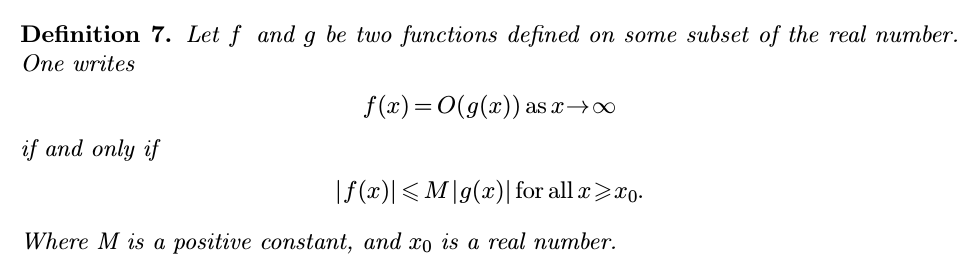
\includegraphics[width=4in]{g.png}}

\end{block}

\end{frame}

\begin{frame}{Speed comparison}

\begin{figure}[h]
  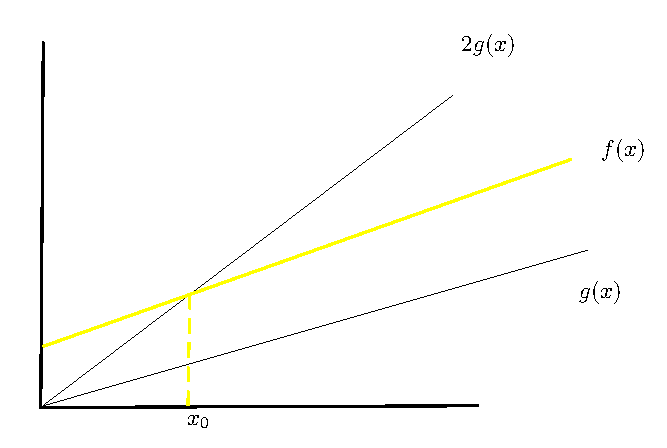
\includegraphics{thesis-8.eps}
\end{figure}

\end{frame}

\begin{frame}{But how does a random number help?}

\begin{block}{Periodicity}

\begin{itemize}
\item
  Input a periodical vector
\item
  Output multiples of period
\item
  Example

  \begin{itemize}
  \itemsep1pt\parskip0pt\parsep0pt
  \item
    Input 100-dimensional vector with period 5.

    \begin{itemize}
    \itemsep1pt\parskip0pt\parsep0pt
    \item
      1,3,5,2,4,1,3,5\ldots{}.5,2,4
    \end{itemize}
  \item
    Output 15, 20

    \begin{itemize}
    \itemsep1pt\parskip0pt\parsep0pt
    \item
      $GCD(15,20)=5$
    \end{itemize}
  \end{itemize}
\end{itemize}

\end{block}

\end{frame}

\section{Shor's algorithm}\label{shors-algorithm}

\begin{frame}{Shor's algorithm step by step}

\begin{itemize}
\item
  Step 1. Choose a random positive integer $m$. Use Euclidean algorithm
  to compute common divisor $gcd(m,N)$ of $m$ and $N$. If greatest
  common divisor $gcd(m.N)\neq 1$,then we have found a non-trivial
  factor of $N$. If, one the other hand, $gcd(m,N) =1$, then proceed to
  step 2.
\item
  Step 2(quantum part). Find the unknown period $P$.
\item
  Step 3. If $P$ is an odd integer, then go to step 1. If $P$ is even,
  then proceed to Step 4.
\item
  Step 4. $(m^{p/2}-1)(m^{p/2}+1)=m^{p}-1=0 \bmod{N}$

  \begin{itemize}
  \itemsep1pt\parskip0pt\parsep0pt
  \item
    If $m^{p/2}+1=0 \bmod{N}$, then go to step 1. If
    $m^{p/2}+1\neq 0 \bmod{N}$, then proceed to step 5.
  \end{itemize}
\item
  Step 5 Use the Euclidean algorithm to compute $d=gcd(m^{p/2}-1,N)$.
\end{itemize}

\end{frame}

\begin{frame}{Quantum part in detail}

\centerline{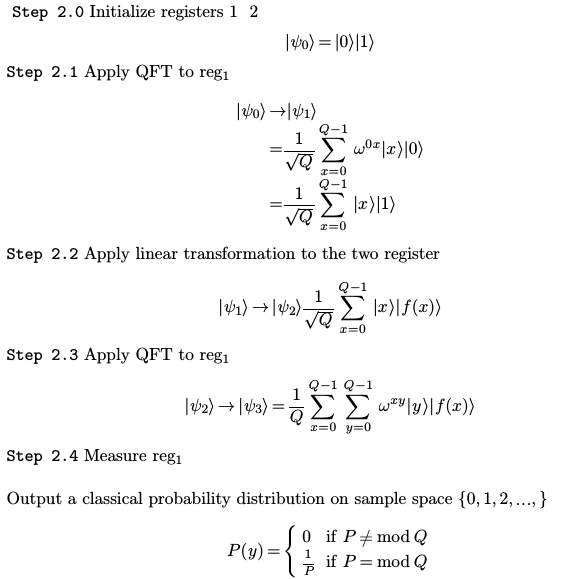
\includegraphics[width=3in]{gg.png}}

\end{frame}

\section{Example}\label{example}

\begin{frame}{A Working example}

\begin{itemize}
\item
  Given $N=91(=7*13)$. Choose $Q=2^{14}=16384$.
\item
  Step 1. Choose a random positive integer $m=3$. Since $gcd(91,3)=1$,
  we proceed to step 2 to find the period of the function $f$ given by
  $f(a)=3^{a}\bmod{91}$.

  \begin{itemize}
  \itemsep1pt\parskip0pt\parsep0pt
  \item
    Unknown to us, $f$ has period 6.
  \end{itemize}
\item
  Step 2. We get period 6 from the quantum part of the Shor's algorithm
\item
  Step 3. Since 6 is an even number, we proceed to Step 4.
\item
  Step 4. Since $3^{P/2}=3^{3}=27\neq 0 \bmod{91}$, we go to Step 5.
\item
  Step 5. With the Euclidean algorithm, we
  compute\[gcd(3^{p/2}-1,91)=gcd(3^{3}-1,91)=gcd(26,91)=13\]
\item
  Exit. Output a non-trivial factor of $N=91$, namely 13.
\end{itemize}

\end{frame}

\begin{frame}{A Working example}

\centerline{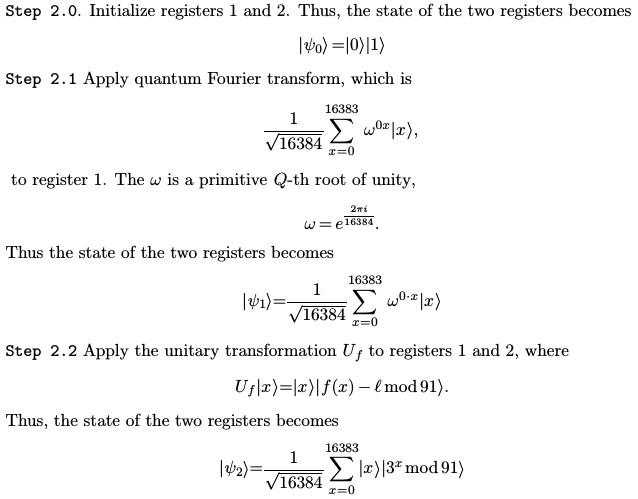
\includegraphics[width=3in]{ggg.png}}

\end{frame}

\begin{frame}{A Working example}

\centerline{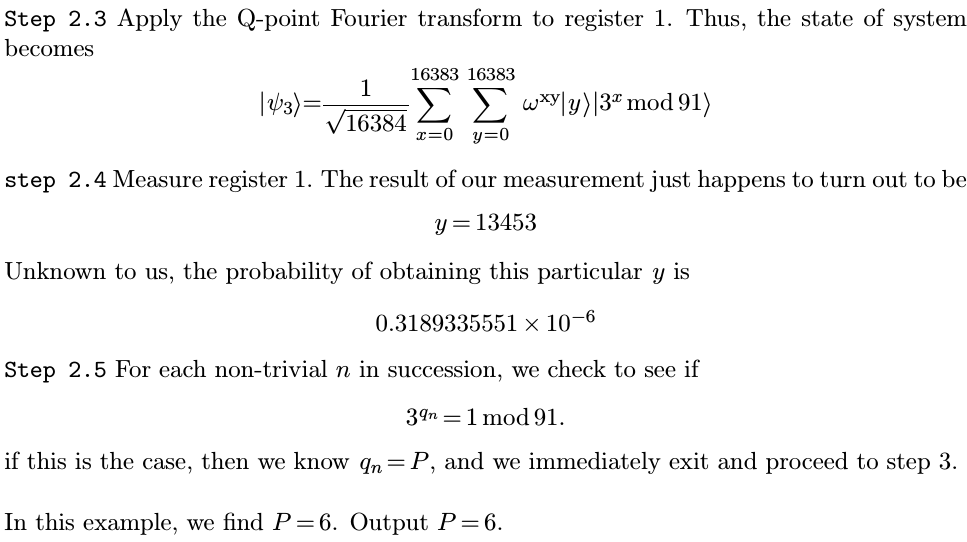
\includegraphics[width=3.2in]{ggggg.png}}

\end{frame}

\section{Q \& A}\label{q-a}

\begin{frame}{Q \& A}

\begin{block}{Q \& A}

\centerline{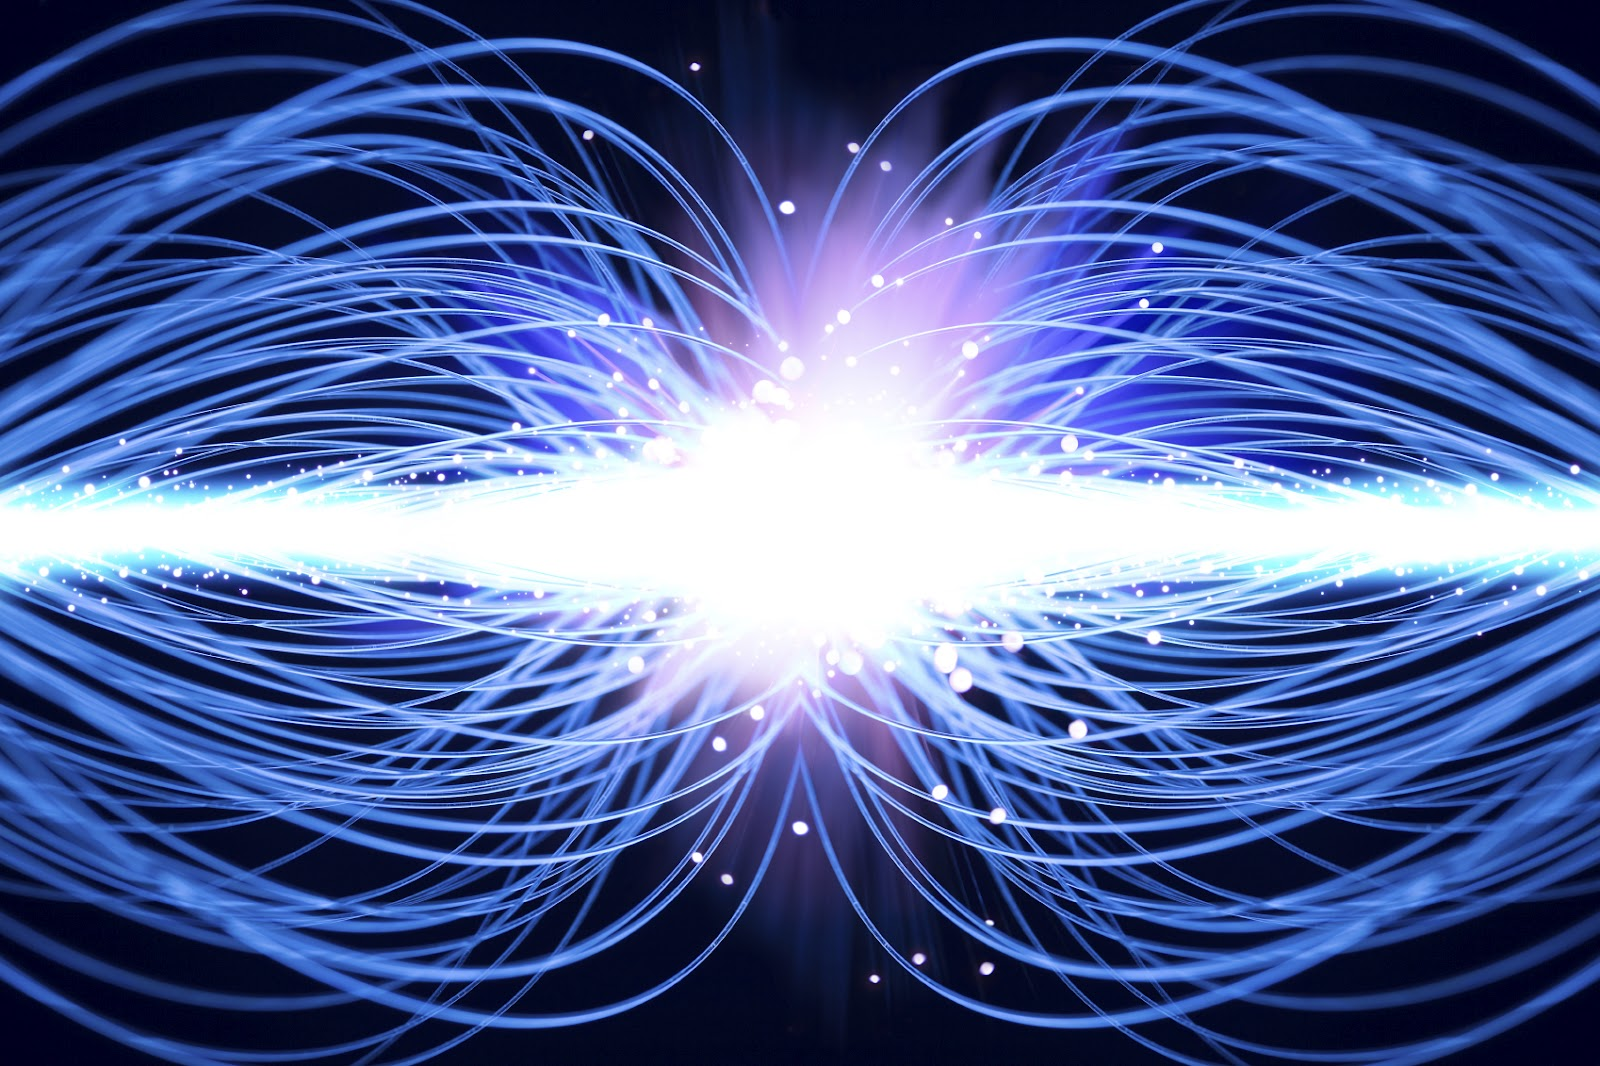
\includegraphics[width=3.8in]{d.jpg}}

\end{block}

\end{frame}
